\begin{frame}
	\myheading{Module 12.1 : Introduction to object detection}
\end{frame}

%%%%%%%%%%%%%%%%%%%%%%%%%%%%%%%%%%%%%%%%%%%%%%%%%%%%%%%%%%%%%%%%%%%%%%%%%%%%%%

\begin{frame}
	\begin{itemize}
		\justifying
		\item So far we have looked at Image Classification
		\item We will now move on to another Image Processing Task - \textit{Object Detection}
	\end{itemize}
\end{frame}

%%%%%%%%%%%%%%%%%%%%%%%%%%%%%%%%%%%%%%%%%%%%%%%%%%%%%%%%%%%%%%%%%%%%%%%%%%%%%%

\begin{frame}
	\begin{overlayarea}{\textwidth}{\textheight}
		
		\vspace{1cm}
		\begin{tikzpicture}
	
	\hspace{+2cm}
	\onslide<1->{
		\node[inner sep=0pt] (A) at (7,4)
		{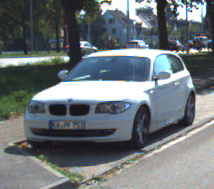
\includegraphics[scale = 0.5]{images/car.png}};
	}

	%\hspace{+2cm}
	\onslide<1->{
		\node[inner sep=0pt] (A) at (13,4)
		{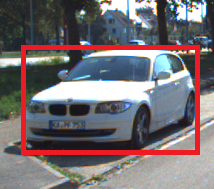
\includegraphics[scale = 1.0]{images/car_boundingbox.png}};
	}

\end{tikzpicture}
		
		% \begin{tabular}{p{1.6cm} p{3.5cm} p{3.5cm} p{3.5cm} }
		% \onslide<2->{ Task} & \onslide<2->{Image classification} & \onslide<4->{Object Detection} & \onslide<6->{Image Segmentation}\\ 
		%  \onslide<3->{Output} & \onslide<3->{Car} & \onslide<5->{Car, exact bounding box containg} & \onslide<7->{Roughly at object boundaries} \\  
		%  \onslide<8->{Annotations} & \onslide<9->{\hspace{+0.1cm}Relatively easier} & \onslide<10->{Relatively easy} & \onslide<11->{Difficult} \\
		% \end{tabular}
		
		\begin{tabular}{p{1.6cm} p{6cm} p{3cm} }
			\onslide<2->{ \textbf{Task}}  & \onslide<2->{Image classification} & \onslide<4->{Object Detection}                       \\ 
			\onslide<3->\textbf{{Output}} & \onslide<3->{Car}                  & \onslide<5->{Car, exact bounding box containing car} \\  
		\end{tabular}
		
	\end{overlayarea}
\end{frame}

%%%%%%%%%%%%%%%%%%%%%%%%%%%%%%%%%%%%%%%%%%%%%%%%%%%%%%%%%%%%%%%%%%%%%%%%%%%%%%

\begin{frame}
	\begin{overlayarea}{\textwidth}{\textheight}
		
		\begin{tikzpicture}
	
	\onslide<1->{
		
		\node[inner sep=0pt] (A) at (3,0)
		{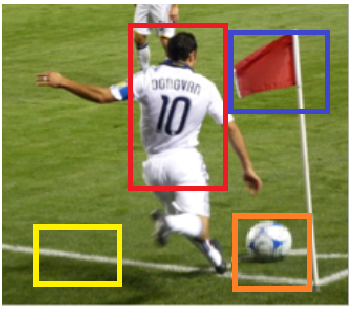
\includegraphics[scale = 0.45]{images/input.png}};
		\draw[black, thick, ->]  (4.5,0) --  (5,0);
	}

	\onslide<2->{
		\node [text width = 30mm] at (6,3){Region proposals};
		\node[inner sep=0pt] (A) at (6,0)
		{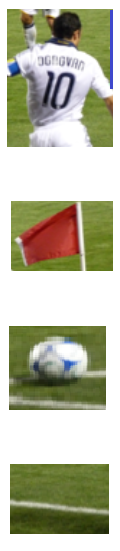
\includegraphics[scale = 0.55]{images/region_proposals.png}};

		\draw[black, thick, ->]  (7,-0.85) --  (7.7,-0.85);
		\draw[black, thick, ->]  (7,-2.15) --  (7.7,-2.15);
		\draw[black, thick, ->]  (7,0.35) --  (7.7,0.35);
		\draw[black, thick, ->]  (7,1.85) --  (7.7,1.85);
	}

	\onslide<4->{
		\tikzstyle{input_neuron}=[circle,draw=red!50,fill=red!10,thick,minimum size=6mm]
		\tikzstyle{hidden_neuron}=[circle,draw=blue!50,fill=cyan!10,thick,minimum size=6mm]
		\tikzstyle{output_neuron}=[circle,draw=green!50,fill=green!10,thick,minimum size=6mm]
		\tikzstyle{cpy_neuron}=[circle,draw=red!50,fill=red!50,thick,minimum size=6mm]
		\tikzstyle{input}=[circle,draw=black!50,fill=black!20,thick,minimum size=6mm]
		\node [text width = 34mm] at (10,3){Feature extraction};
		\node [input_neuron] (neuron51) at (8.5,1.85) {} ;
		\node [input_neuron] (neuron52) at (9.5,1.85)  {};
		\node [input_neuron] (neuron53) at (10.5,1.85)  {};
		\node [input_neuron] (neuron54) at (11.5,1.85)  {};
		\node [text width = 5mm] at (8.7,1.1){$x_1$};
		\node [text width = 5mm] at (9.7,1.1){$x_2$};
		\node [text width = 5mm] at (10.7,1.1){$\dots$};
		\node [text width = 5mm] at (11.7,1.1){$x_d$};
		\draw[red!100,thick,solid,rounded corners=15pt] (8,2.35) rectangle (12,1.35);
	}
	
	\onslide<5->{
		\node [text width = 25mm] at (14.5,3){\ \ \ Classifier};
		\node [text width = 10mm] at (12.8,2.6){person};
		\node [text width = 10mm] at (14,2.6){flag};
		\node [text width = 10mm] at (15,2.6){ball};
		\node [text width = 10mm] at (16,2.6){none};
		\draw[black, thick, ->] (12.1,1.85) --  (12.4,1.85);
		\node [output_neuron] (neuron51) at (13,1.85) {} ;
		\node [output_neuron] (neuron52) at (14,1.85)  {};
		\node [output_neuron] (neuron53) at (15,1.85)  {};
		\node [output_neuron] (neuron54) at (16,1.85)  {};
		\draw[red!100,thick,solid] (12.5,2.35) rectangle (16.5,1.35);
		\node [cpy_neuron] (neuron01) at (13,1.85) {};
	}

	\onslide<4->{
		\node [input_neuron] (neuron51) at (8.5,0.35) {} ;
		\node [input_neuron] (neuron52) at (9.5,0.35)  {};
		\node [input_neuron] (neuron53) at (10.5,0.35)  {};
		\node [input_neuron] (neuron54) at (11.5,0.35)  {};
		
		\draw[red!100,thick,solid,rounded corners=15pt] (8,0.85) rectangle (12,-0.15);
	} 
	
	\onslide<5->{
		
		\draw[black, thick, ->] (12.1,0.35) --  (12.4,0.35);

		\node [output_neuron] (neuron51) at (13,0.35) {} ;
		\node [output_neuron] (neuron52) at (14,0.35)  {};
		\node [output_neuron] (neuron53) at (15,0.35)  {};
		\node [output_neuron] (neuron54) at (16,0.35)  {};
		
		\draw[red!100,thick,solid] (12.5,-0.15) rectangle (16.5,0.85);
		
		\node [cpy_neuron] (neuron01) at (14,0.35) {};
	}
	
	
	\onslide<4->{
		
		\node [input_neuron] (neuron51) at (8.5,-0.85) {} ;
		\node [input_neuron] (neuron52) at (9.5,-0.85)  {};
		\node [input_neuron] (neuron53) at (10.5,-0.85)  {};
		\node [input_neuron] (neuron54) at (11.5,-0.85)  {};
		
		\draw[red!100,thick,solid,rounded corners=15pt] (8,-1.35) rectangle (12,-0.35);
	} 
	
	
	\onslide<5->{
		
		\draw[black, thick, ->] (12.1,-0.85) --  (12.4,-0.85);

		\node [output_neuron] (neuron51) at (13,-0.85) {} ;
		\node [output_neuron] (neuron52) at (14,-0.85)  {};
		\node [output_neuron] (neuron53) at (15,-0.85)  {};
		\node [output_neuron] (neuron54) at (16,-0.85)  {};
		
		\draw[red!100,thick,solid] (12.5,-1.35) rectangle (16.5,-0.35);
		
		\node [cpy_neuron] (neuron01) at (15,-0.85) {};
	}
	
	\onslide<4->{
		\node [input_neuron] (neuron51) at (8.5,-2.15) {} ;
		\node [input_neuron] (neuron52) at (9.5,-2.15)  {};
		\node [input_neuron] (neuron53) at (10.5,-2.15)  {};
		\node [input_neuron] (neuron54) at (11.5,-2.15)  {};
		
		\draw[red!100,thick,solid,rounded corners=15pt] (8,-2.65) rectangle (12,-1.65);
	} 
	
	
	\onslide<5->{
		
		\draw[black, thick, ->] (12.1,-2.15) --  (12.4,-2.15);
		\node [output_neuron] (neuron51) at (13,-2.15) {} ;
		\node [output_neuron] (neuron52) at (14,-2.15)  {};
		\node [output_neuron] (neuron53) at (15,-2.15)  {};
		\node [output_neuron] (neuron54) at (16,-2.15)  {};
		
		\draw[red!100,thick,solid] (12.5,-2.65) rectangle (16.5,-1.65);
		
		\node [cpy_neuron] (neuron01) at (16,-2.15) {};
	}
\end{tikzpicture}
		\begin{itemize}
			\justifying
			\only<1-2> {\item<1-> Let us see a typical pipeline for \it{object detection}
				\item<2-> It starts with a region proposal stage where we identify potential regions which may contain objects
			}
			\only<3-4>{
				\item<3-> We could think of these regions as mini-images
				\item<4-> We extract features(SIFT, HOG, CNNs) from these mini-images
			}
			\only<5->{
				\item<5-> Pass these through a standard image classifer to determine the class
			}
		\end{itemize}
	\end{overlayarea}     
	
\end{frame}

%%%%%%%%%%%%%%%%%%%%%%%%%%%%%%%%%%%%%%%%%%%%%%%%%%%%%%%%%%%%%%%%%%%%%%%%%%%%%%

\begin{frame}
	\begin{overlayarea}{\textwidth}{\textheight}
		\begin{tikzpicture}
	\onslide<1->{
		\node[inner sep=0pt] (A) at (3,0)
		{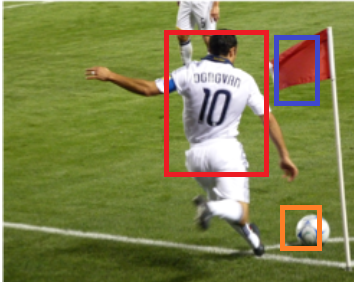
\includegraphics[scale = 0.45]{images/input_2.png}};
		\draw[black, thick, ->]  (4.5,0) --  (5,0);
	}

	\onslide<1->{
		\node [text width = 30mm] at (6,3){Region proposals};
		\node[inner sep=0pt] (A) at (6,0)
		{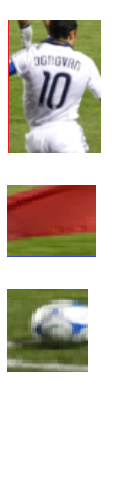
\includegraphics[scale = 0.65]{images/region_proposals_2.png}};

		\node [text width = 10mm] at (6.9,-0.8){$h$};
		\node [text width = 10mm] at (6.2,-1.6){$w$};
		
		\node [text width = 10mm] at (7.1,1.9){$h$};
		\node [text width = 10mm] at (6.2,0.9){$w$};
		
		
		\node [text width = 10mm] at (7.1,0.4){$h$};
		\node [text width = 10mm] at (6.2,-0.3){$w$};
	}

	\onslide<3->{
		\tikzstyle{input_neuron}=[circle,draw=red!50,fill=red!10,thick,minimum size=6mm]
		\tikzstyle{hidden_neuron}=[circle,draw=blue!50,fill=cyan!10,thick,minimum size=6mm]
		\tikzstyle{output_neuron}=[circle,draw=green!50,fill=green!10,thick,minimum size=6mm]
		\tikzstyle{cpy_neuron}=[circle,draw=red!50,fill=red!50,thick,minimum size=6mm]
		\tikzstyle{input}=[circle,draw=black!50,fill=black!20,thick,minimum size=6mm]
		\node [text width = 34mm] at (10,3){Feature extraction};
		\node [input_neuron] (neuron51) at (8.5,1.85) {} ;
		\node [input_neuron] (neuron52) at (9.5,1.85)  {};
		\node [input_neuron] (neuron53) at (10.5,1.85)  {};
		\node [input_neuron] (neuron54) at (11.5,1.85)  {};
		\node [text width = 5mm] at (8.7,1.1){$x_1$};
		\node [text width = 5mm] at (9.7,1.1){$x_2$};
		\node [text width = 5mm] at (10.7,1.1){$\dots$};
		\node [text width = 5mm] at (11.7,1.1){$x_d$};
		\draw[red!100,thick,solid,rounded corners=15pt] (8,2.35) rectangle (12,1.35);
	}  
	
	\onslide<2->{
		\node [text width = 50mm] at (14.5,3){Bounding box regression};
		\node[inner sep=0pt] (A) at (13.0,2)
		{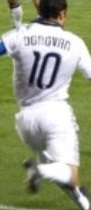
\includegraphics[scale = 0.45]{images/man_corrected.jpg}};
		\node [text width = 10mm] at (14.0,1.7){$h^*$};
		\node [text width = 10mm] at (13.4,1){$w^*$};
		
	}


	\onslide<3->{
		\node [input_neuron] (neuron51) at (8.5,0.35) {} ;
		\node [input_neuron] (neuron52) at (9.5,0.35)  {};
		\node [input_neuron] (neuron53) at (10.5,0.35)  {};
		\node [input_neuron] (neuron54) at (11.5,0.35)  {};
		
		\draw[red!100,thick,solid,rounded corners=15pt] (8,0.85) rectangle (12,-0.15);
	} 
	
	\onslide<2->{
		\node[inner sep=0pt] (A) at (13.0,0.35)
		{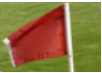
\includegraphics[scale = 0.5]{images/flag_corrected.png}};
		\node [text width = 10mm] at (14.0,0.43){$h^*$};
		\node [text width = 10mm] at (13.4,-0.2){$w^*$};
		
	}
	
	\onslide<3->{
		
		\node [input_neuron] (neuron51) at (8.5,-0.85) {} ;
		\node [input_neuron] (neuron52) at (9.5,-0.85)  {};
		\node [input_neuron] (neuron53) at (10.5,-0.85)  {};
		\node [input_neuron] (neuron54) at (11.5,-0.85)  {};
		
		\draw[red!100,thick,solid,rounded corners=15pt] (8,-1.35) rectangle (12,-0.35);
	} 
	
	\onslide<2->{
		\node[inner sep=0pt] (A) at (13.0,-0.88)
		{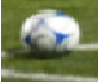
\includegraphics[scale = 0.45]{images/ball_corrected.png}};
		\node [text width = 10mm] at (14.0,-0.8){$h^*$};
		\node [text width = 10mm] at (13.4,-1.35){$w^*$};
	} 
	
	\onslide<3->{
		\draw[black, thick, ->]  (7,-0.85) --  (7.7,-0.85);
		%\draw[black, thick, ->]  (7,-2.15) --  (7.7,-2.15);
		\draw[black, thick, ->]  (7,0.35) --  (7.7,0.35);
		\draw[black, thick, ->]  (7,1.85) --  (7.7,1.85);
		
		\draw[black, thick, ->] (12.1,1.85) --  (12.4,1.85);
		\draw[black, thick, ->] (12.1,0.35) --  (12.4,0.35);
		\draw[black, thick, ->] (12.1,-0.85) --  (12.4,-0.85);
	}
	
	
\end{tikzpicture}
		
		\begin{itemize}
			\justifying
			\item<1-> In addition we would also like to correct the proposed bounding boxes
			\item<2-> This is posed as a regression problem (for example, we would like to predict $w^*$, $h^*$ from the proposed $w$ and $h$)
		\end{itemize}
		
	\end{overlayarea}     
\end{frame}

%%%%%%%%%%%%%%%%%%%%%%%%%%%%%%%%%%%%%%%%%%%%%%%%%%%%%%%%%%%%%%%%%%%%%%%%%%%%%%

\begin{frame}
	\begin{columns}
		\column{0.5\textwidth}
		\begin{overlayarea}{\textwidth}{\textheight}
			
			\tikzstyle{input_neuron}=[circle,draw=red!50,fill=red!10,thick,minimum size=4mm]
\tikzstyle{hidden_neuron}=[circle,draw=blue!50,fill=cyan!10,thick,minimum size=4mm]
\tikzstyle{output_neuron}=[circle,draw=green!50,fill=green!10,thick,minimum size=4mm]
\tikzstyle{cpy_neuron}=[circle,draw=red!50,fill=red!50,thick,minimum size=4mm]
\tikzstyle{input}=[circle,draw=black!50,fill=black!20,thick,minimum size=4mm]

\begin{tikzpicture}[scale=0.5, transform shape]
	
	\onslide<1->{
		\node [text width = 30mm] at (2.5,3){Region proposals};
		\node[inner sep=0pt] (A) at (2.5,1.8)
		{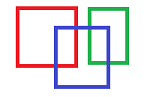
\includegraphics[scale = 0.9]{images/bboxes.png}};

		\node [text width = 34mm] at (6.5,3){Feature extraction};
		\node[inner sep=0pt] (A) at (6.5,2)
		{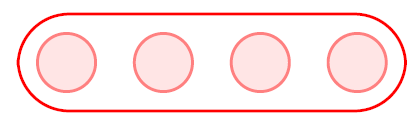
\includegraphics[scale = 0.5]{images/feature.PNG}};
		
		\node [text width = 25mm] at (11.5,3){Classifier};
		\node[inner sep=0pt] (A) at (11.0,2)
		{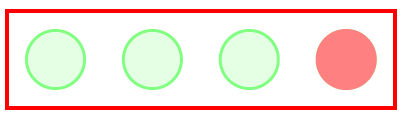
\includegraphics[scale = 0.5]{images/classification.PNG}};
	}
	
	\onslide<1->{
		\node [text width = 25mm] at (0,0){Pre 2012};
		\node[inner sep=0pt] (A) at (2.5,0.2)
		{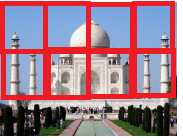
\includegraphics[scale = 0.6]{images/pre_2012.png}};
		\node[inner sep=0pt] (B) at (5.9,0.2)
		{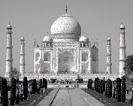
\includegraphics[scale = 0.8]{images/sift.PNG}};
		\node[inner sep=0pt] (C) at (8,0.2)
		{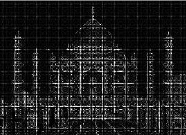
\includegraphics[scale = 0.6]{images/hog.PNG}};
		\node[inner sep=0pt] (D) at (11,0.4)
		{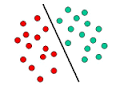
\includegraphics[scale = 0.45]{images/svm.PNG}};
	}
	

	\onslide<1->{
		\node [text width = 25mm] at (0,-1.5){RCNN};
		\node[inner sep=0pt] (A) at (2.5,-1.3)
		{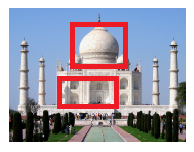
\includegraphics[scale = 0.6]{images/rcnn_bbox.png}};
		\node[inner sep=0pt] (B) at (6.8,-1.4)
		{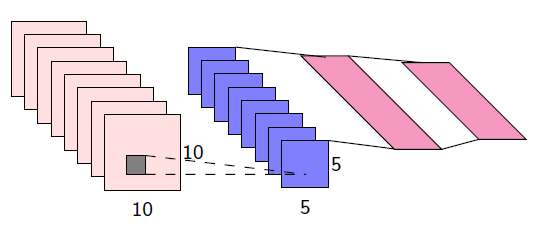
\includegraphics[scale = 0.4]{images/cnn.PNG}};
		\node[inner sep=0pt] (D) at (11,-1.2)
		{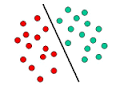
\includegraphics[scale = 0.45]{images/svm.PNG}};
	}
	
	\onslide<1->{
		\node [text width = 25mm] at (0,-3){
		Fast RCNN};
		\node[inner sep=0pt] (A) at (2.5,-2.8)
		{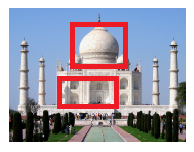
\includegraphics[scale = 0.6]{images/rcnn_bbox.png}};
		\node[inner sep=0pt] (B) at (8.8,-2.9)
		{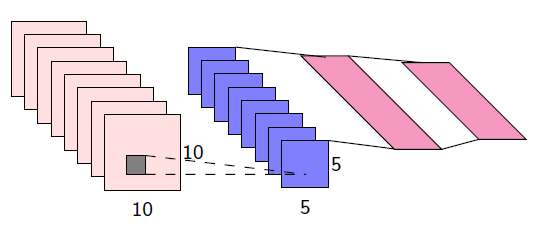
\includegraphics[height=1.5cm,width=6cm]{images/cnn.PNG}};
		%\node[inner sep=0pt] (D) at (11,-2.8)
		%{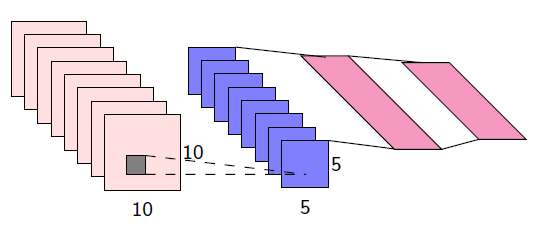
\includegraphics[scale = 0.4]{images/cnn.PNG}};
	}
	
	\onslide<1->{
		\node [text width = 25mm] at (0,-4.8){Faster RCNN};}
	\onslide<2->{\node[inner sep=0pt] (A) at (3,-4.6)
		{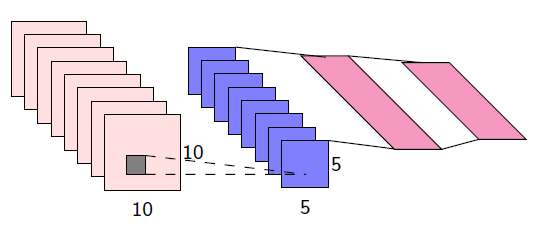
\includegraphics[scale = 0.4]{images/cnn.PNG}};}
	\onslide<3->{\node[inner sep=0pt] (B) at (8.8,-4.6)
		{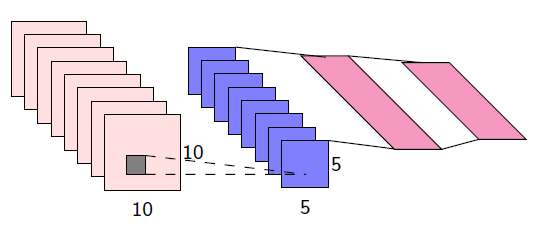
\includegraphics[height=1.5cm,width=6cm]{images/cnn.PNG}};}
	%\onslide<4->{\node[inner sep=0pt] (D) at (11,-4.5)
	%	{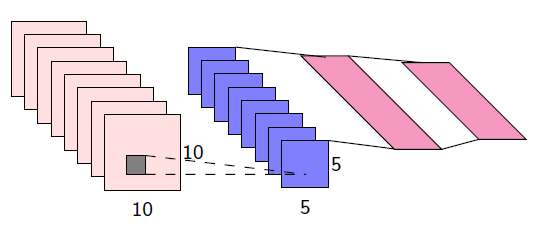
\includegraphics[scale = 0.4]{images/cnn.PNG}};}
\end{tikzpicture}
		\end{overlayarea}
		\column{0.5\textwidth}
		\begin{overlayarea}{\textwidth}{\textheight}
			\begin{itemize}
				\justifying
				\item<1-> Let us see how these three components have evolved over time
				\item<2-> Propose all possible regions in the image of varying sizes (almost brute force)
				\item<3-> Use handcrafted features (SIFT, HOG)
				\item<4-> Train a linear classifier using these features
				\item<5-> We will now see three algorithms that progressively improve these components 
			\end{itemize}
		\end{overlayarea}
	\end{columns}
\end{frame}

